% !TEX encoding = UTF-8 Unicode
%!TEX root = ../Main/thesis.tex
% !TEX spellcheck = en-US
%%=========================================
\documentclass[../Main/thesis.tex]{subfiles}
\begin{document}
\chapter{Second Iteration  - First prototype}
\label{ch:development-1}
This chapter describes the second iteration of the development.
In this iteration a prototype of both the Android application and the back-end was developed.
The iteration ended with a demonstration and test of the prototypes for Øygarden Fire and Rescue.

\section{Android application}
The goal for this iteration was to implement the Bluetooth data collecting functionality, and the possibility to upload a completed session to the server, using the design proposed in Chapter~\ref{ch:requirements}.

This version of the app is shown in Figure~\ref{fig:app-first-prototype}.
The first screen in the application (see Figure~\ref{fig:app-first-prototype-sessionlist}) contains a list of available sessions. 
Each session is represented with a name and the name of the person who is supposed to use that session.
When a smoke diver is getting ready for the exercise he chooses the appropriate session from the list which takes him to the next screen.

The second screen in the app (see Figure~\ref{fig:app-first-prototype-trackingactivity}) tells the user that the app is not currently tracking and has a blue play-button and instructions telling the user to press the button to start the tracking.
When a user presses the play-button a dialog-box is shown asking for confirmation that the user want to start the tracking. 
If the user confirms he is taken to the third screen (see Figure~\ref{fig:app-first-prototype-tracking}) and the app starts searching for BLE-signals.
Every time the app receives a BLE-signal it stores the signal-strength, identifiers of the beacon transmitting the signal, data from the gyroscope and accelerometer in the phone, and a timestamp, as a datapoint in the current session.
When the user has finished the tracking and presses the stop-button, a new dialog appears to confirm that the user want to end the tracking.
If the user confirms all the recorded data is uploaded to the server for processing, a upload-dialog is shown (see Figure~\ref{fig:app-first-prototype-upload}).
After the uploading is finished the user is taken back to the list of available sessions.

\begin{figure}[h]
	\centering
	\begin{subfigure}{0.2\textwidth}
		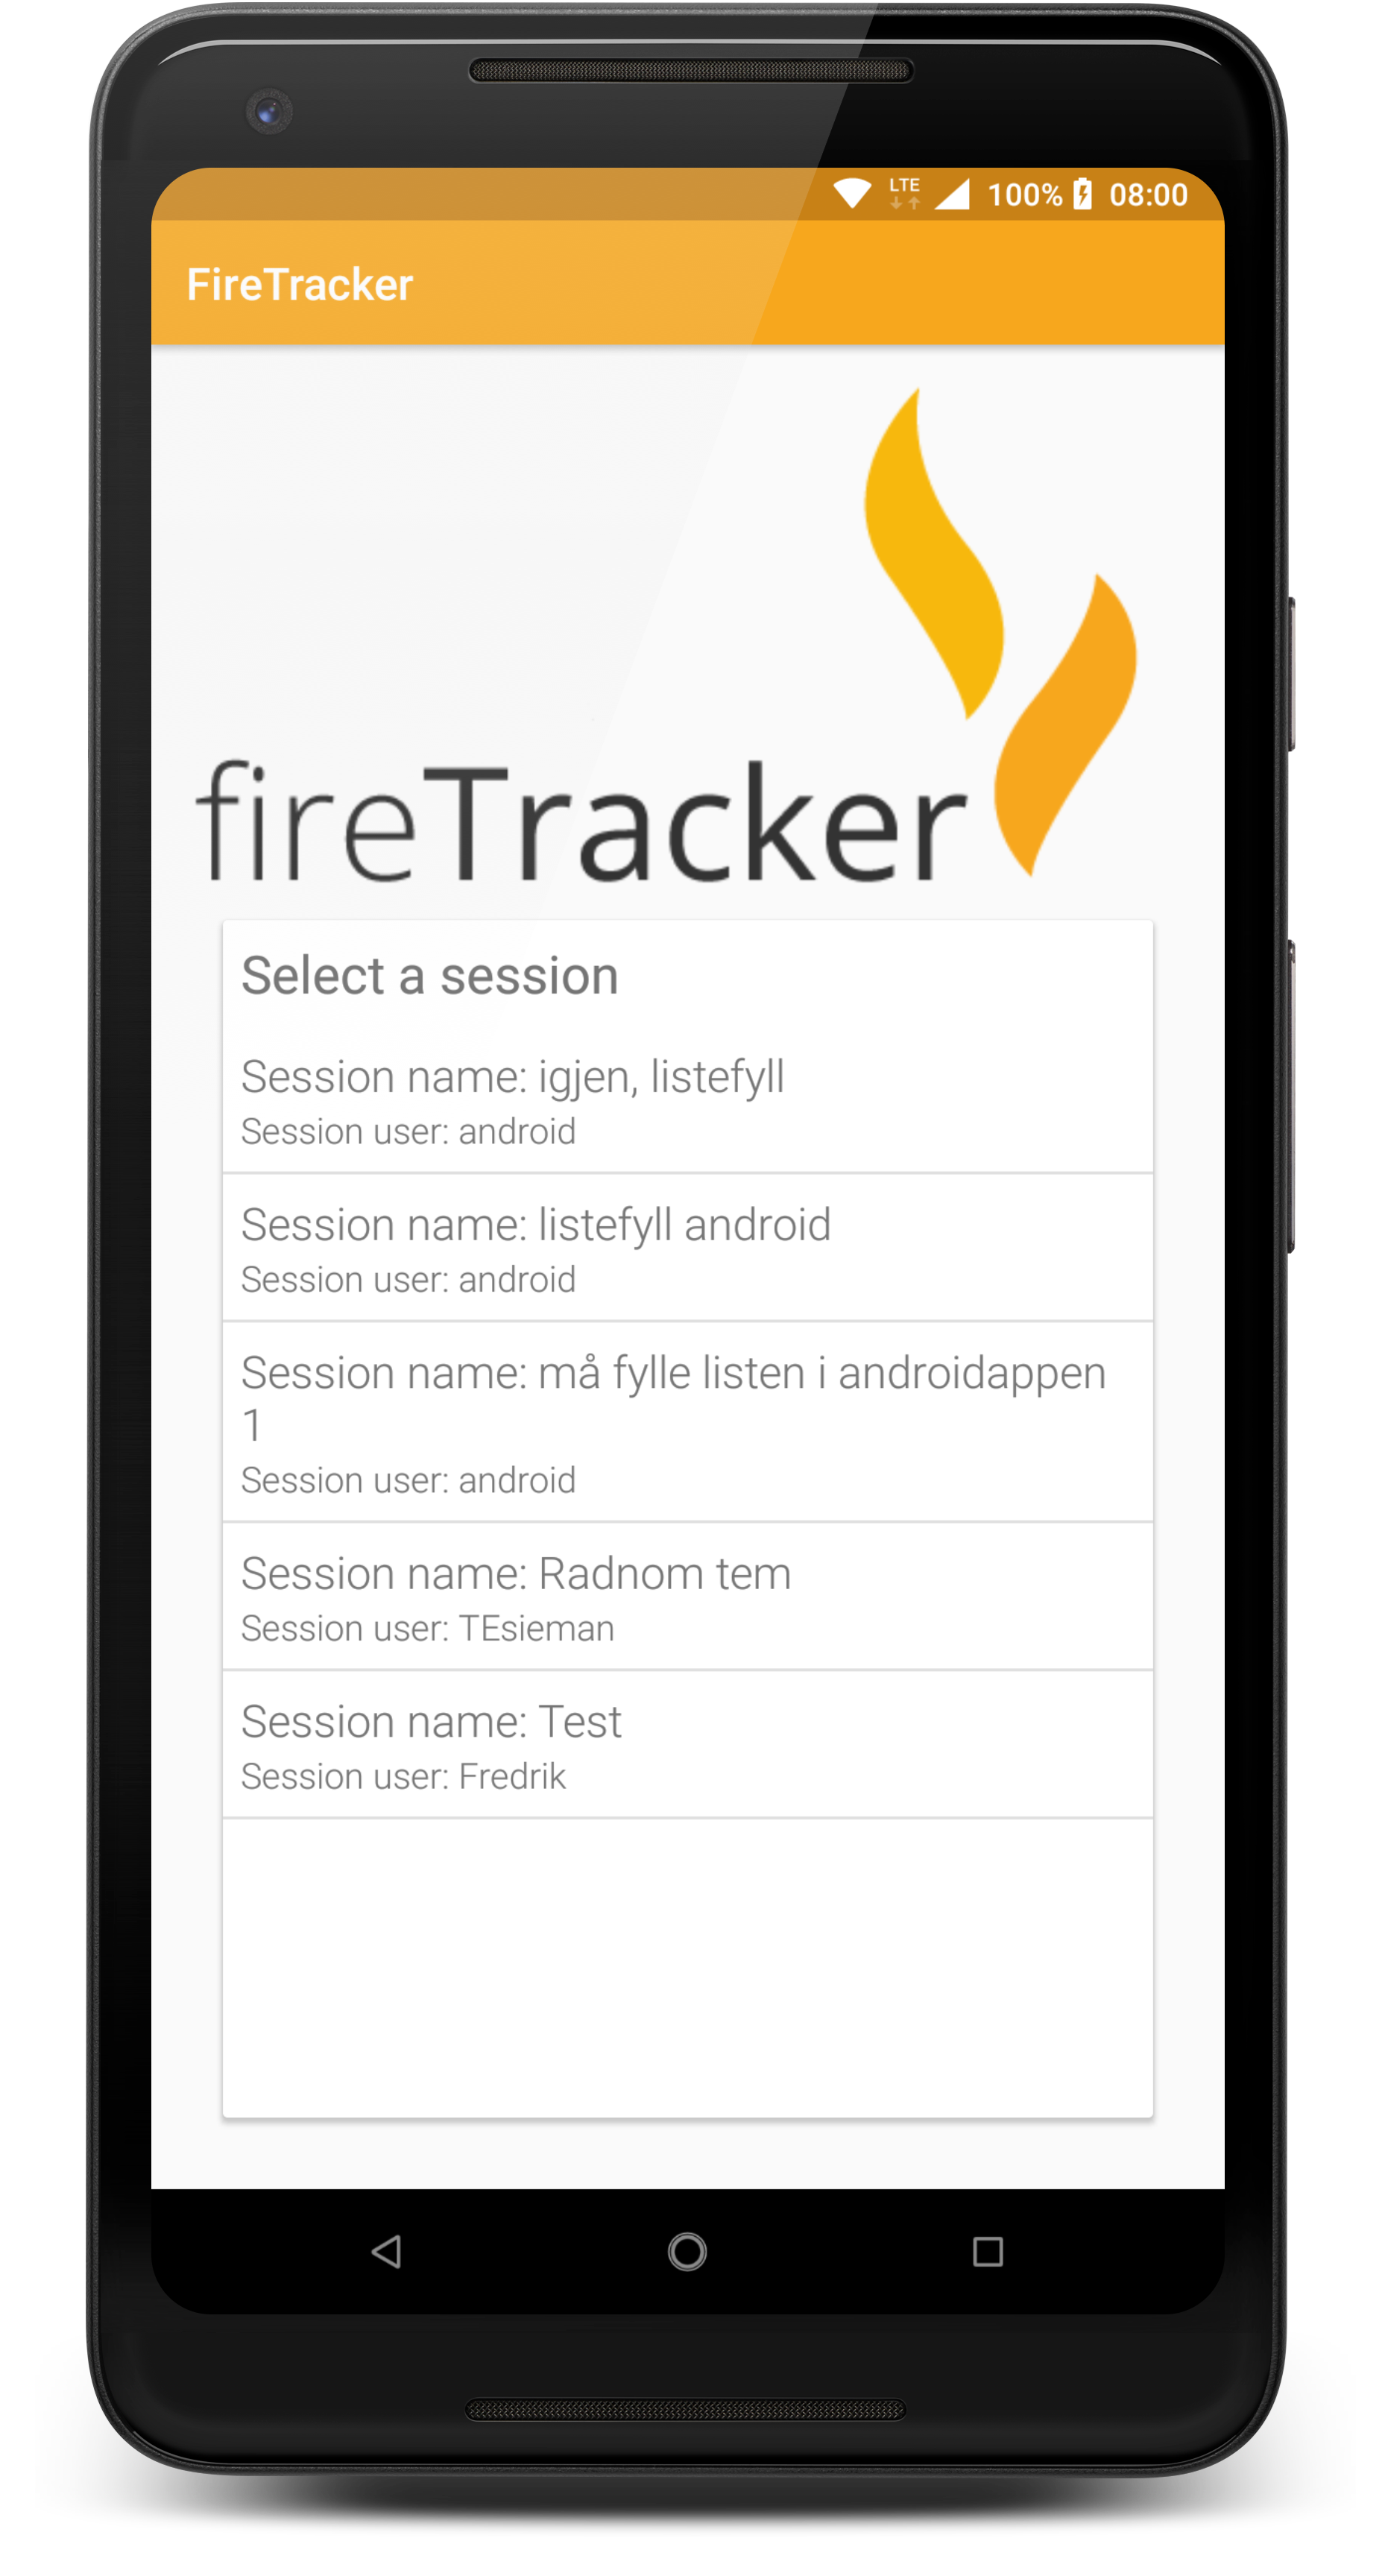
\includegraphics[width=\textwidth]{../fig/firetracker_app_old_1}
		\caption{List of sessions}
		\label{fig:app-first-prototype-sessionlist}
	\end{subfigure}
	\begin{subfigure}{0.2\textwidth}
		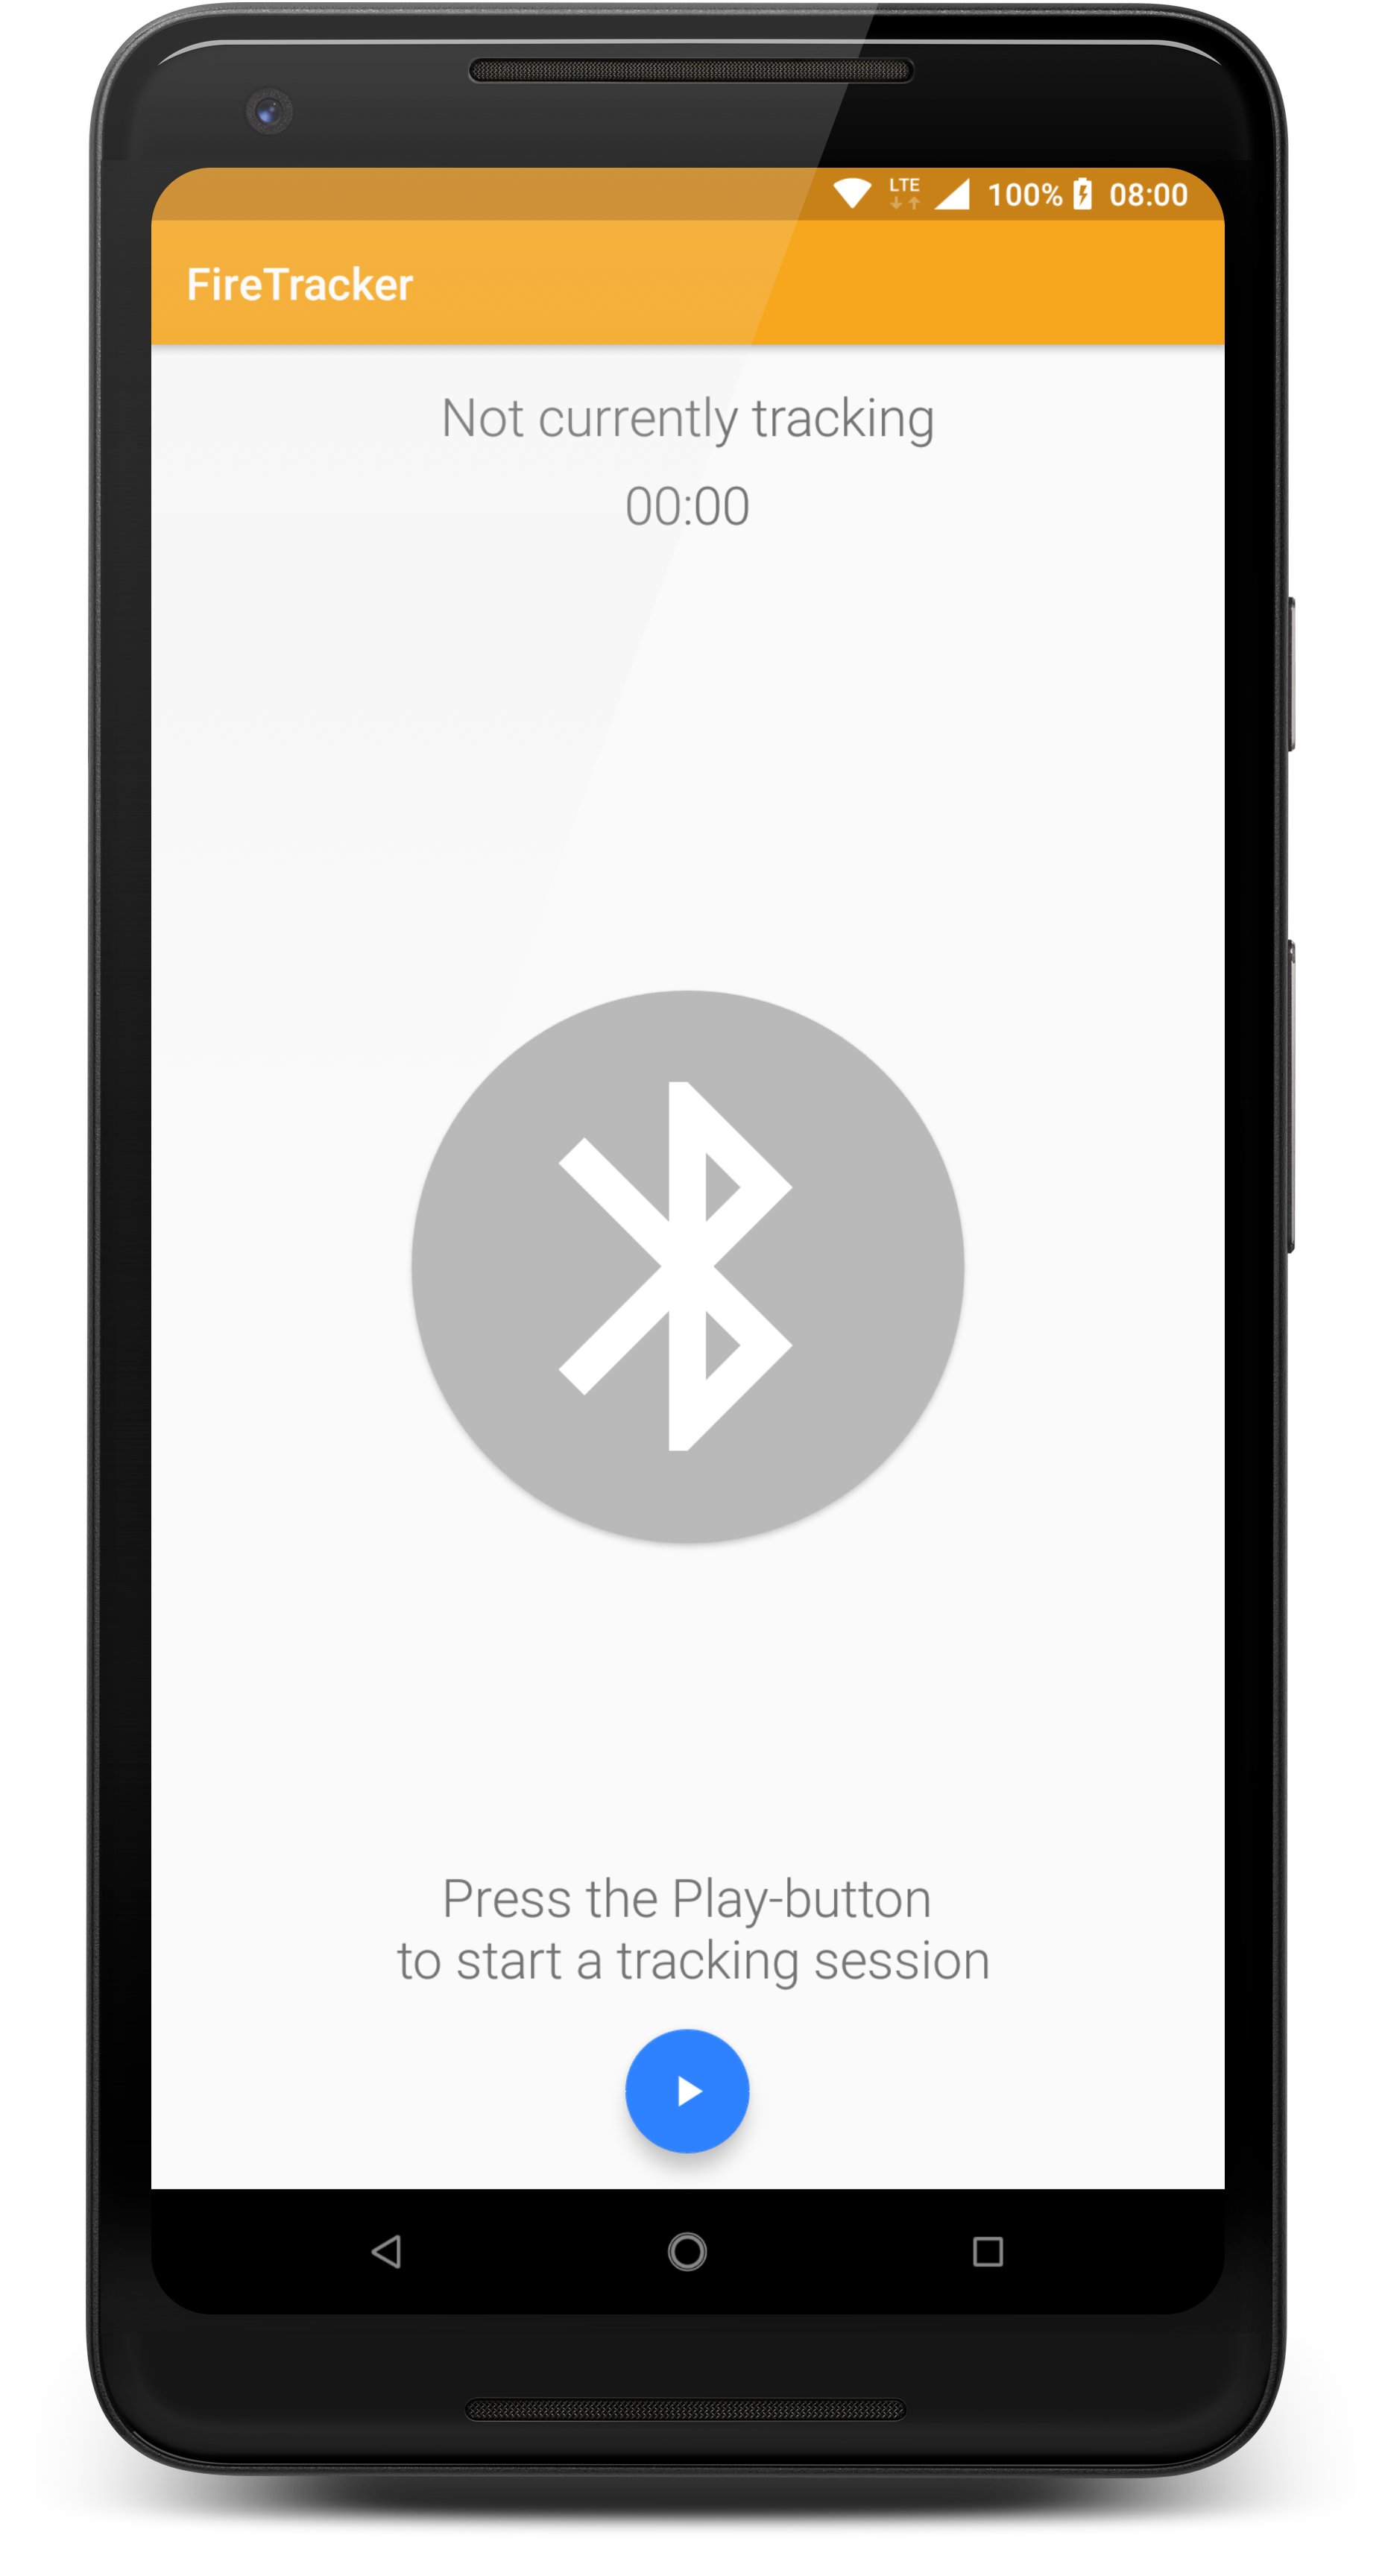
\includegraphics[width=\textwidth]{../fig/firetracker_app_old_2}
		\caption{Tracking activity}
		\label{fig:app-first-prototype-trackingactivity}
	\end{subfigure}
	\begin{subfigure}{0.2\textwidth}
		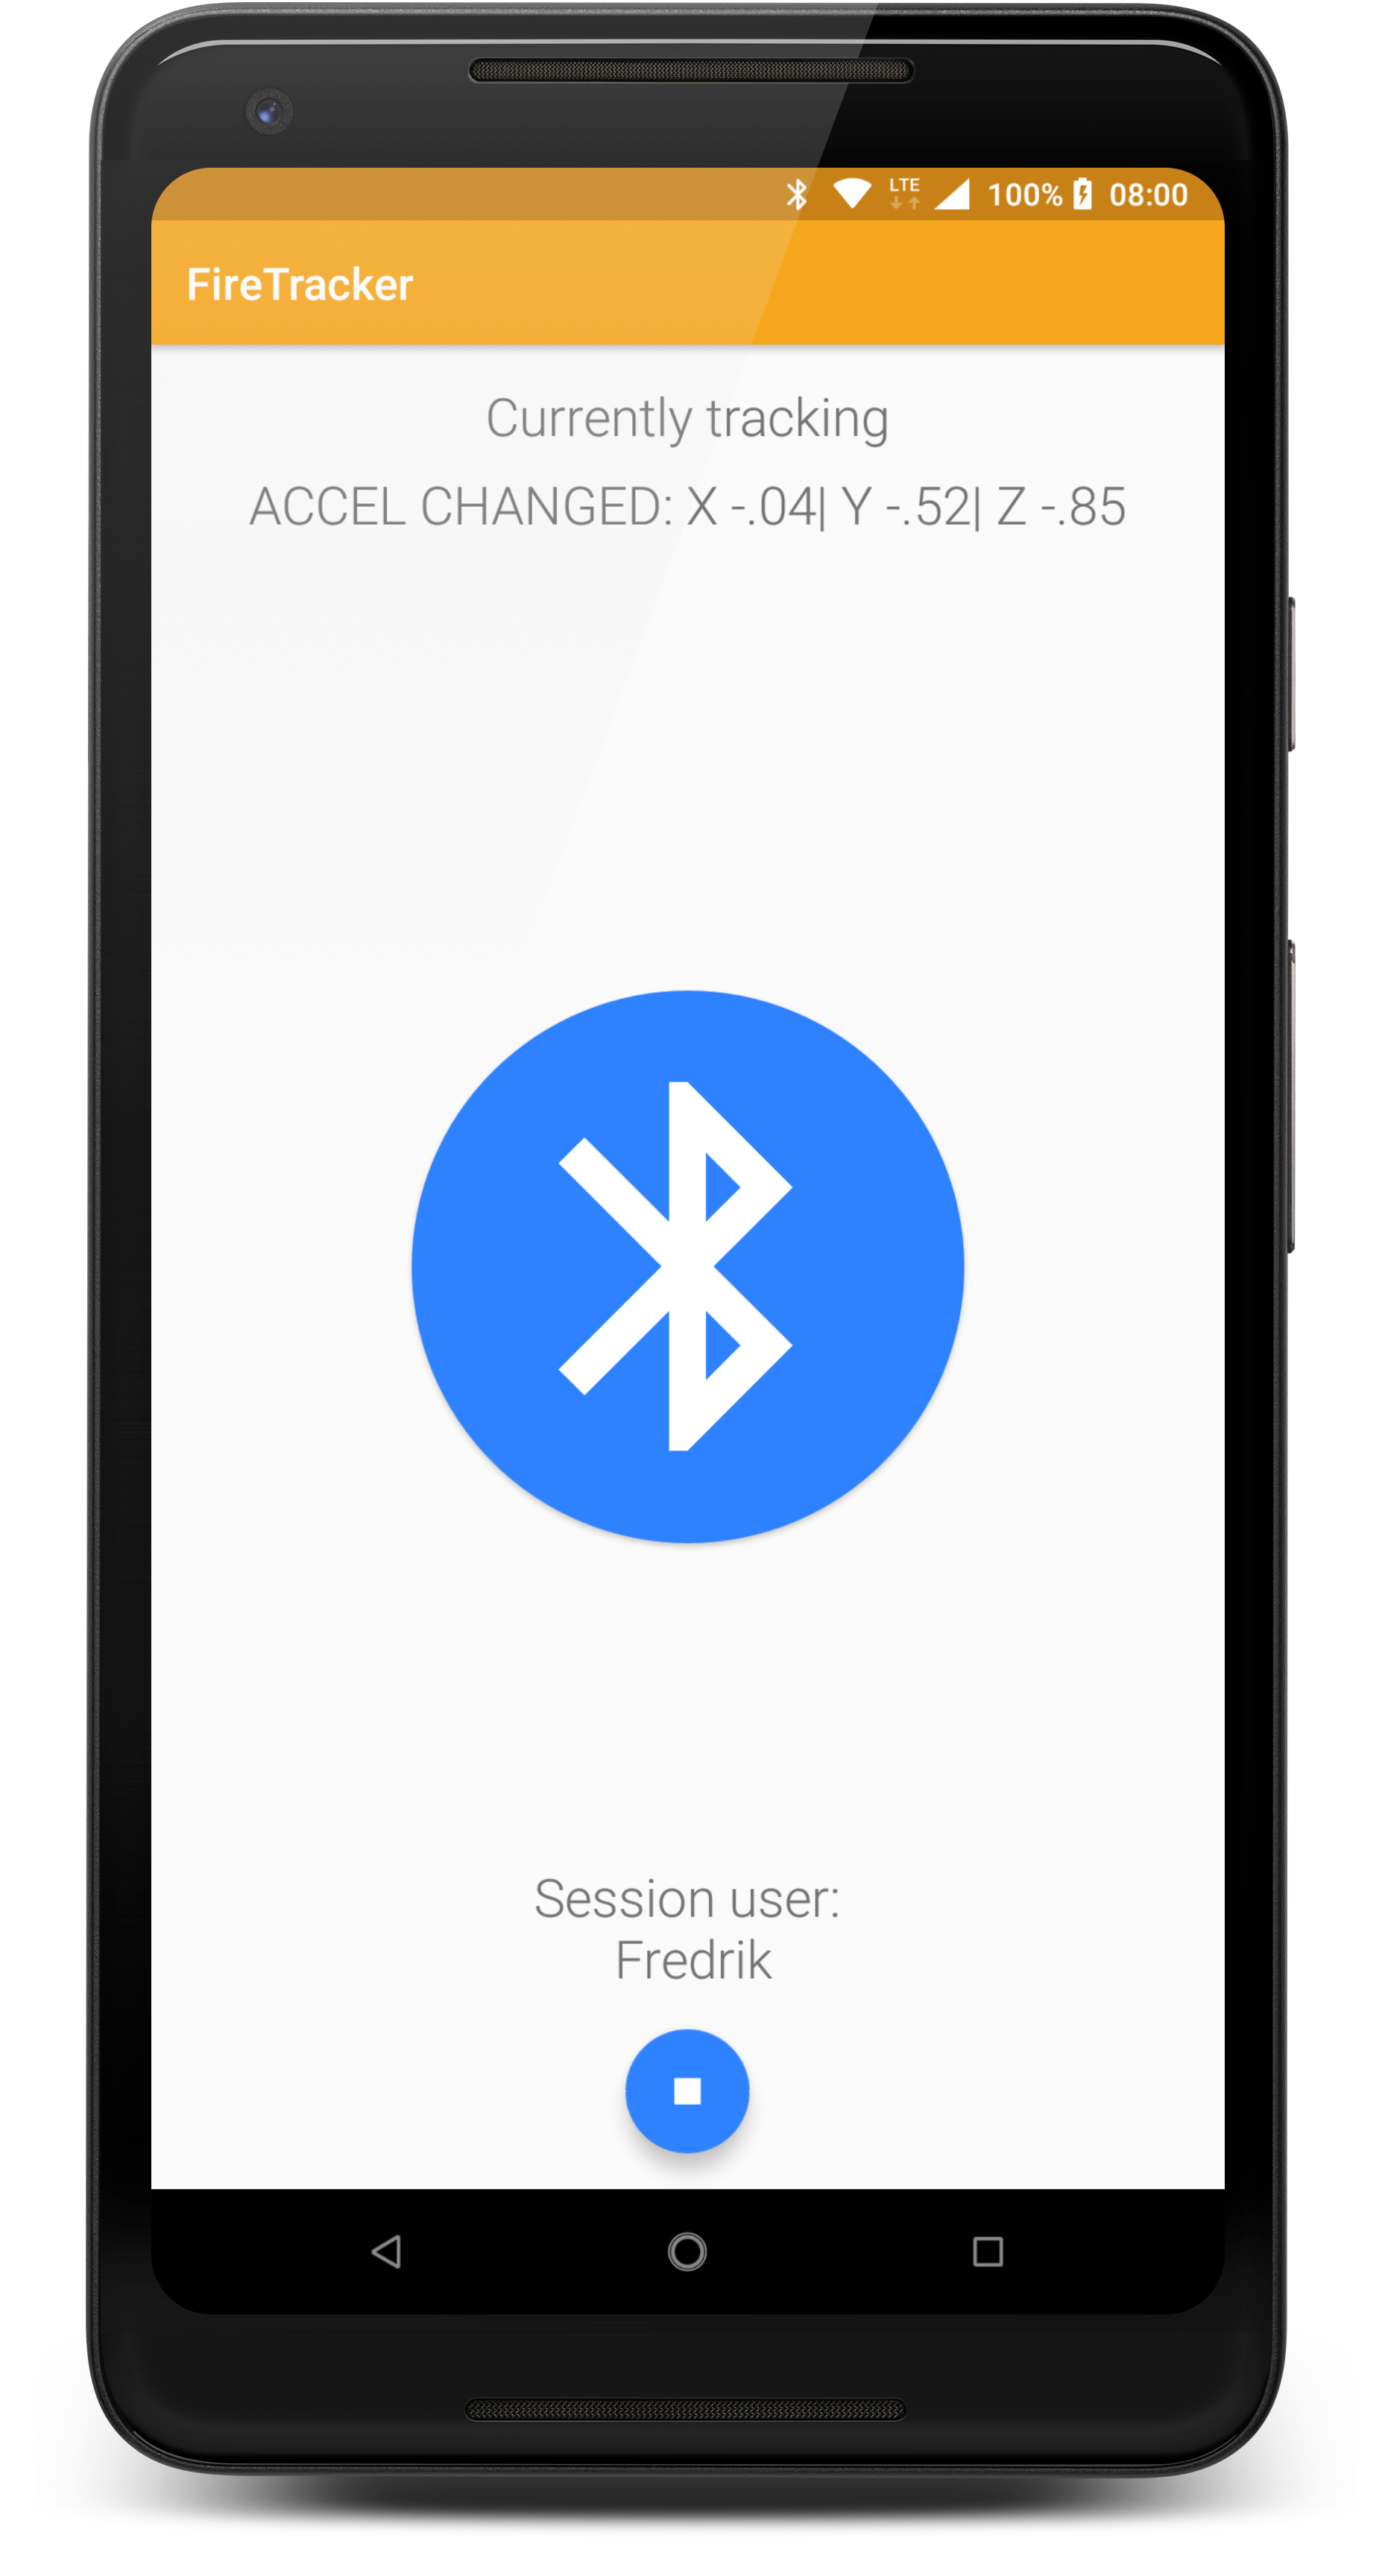
\includegraphics[width=\textwidth]{../fig/firetracker_app_old_3}
		\caption{Active tracking}
		\label{fig:app-first-prototype-tracking}
	\end{subfigure}
	\begin{subfigure}{0.2\textwidth}
		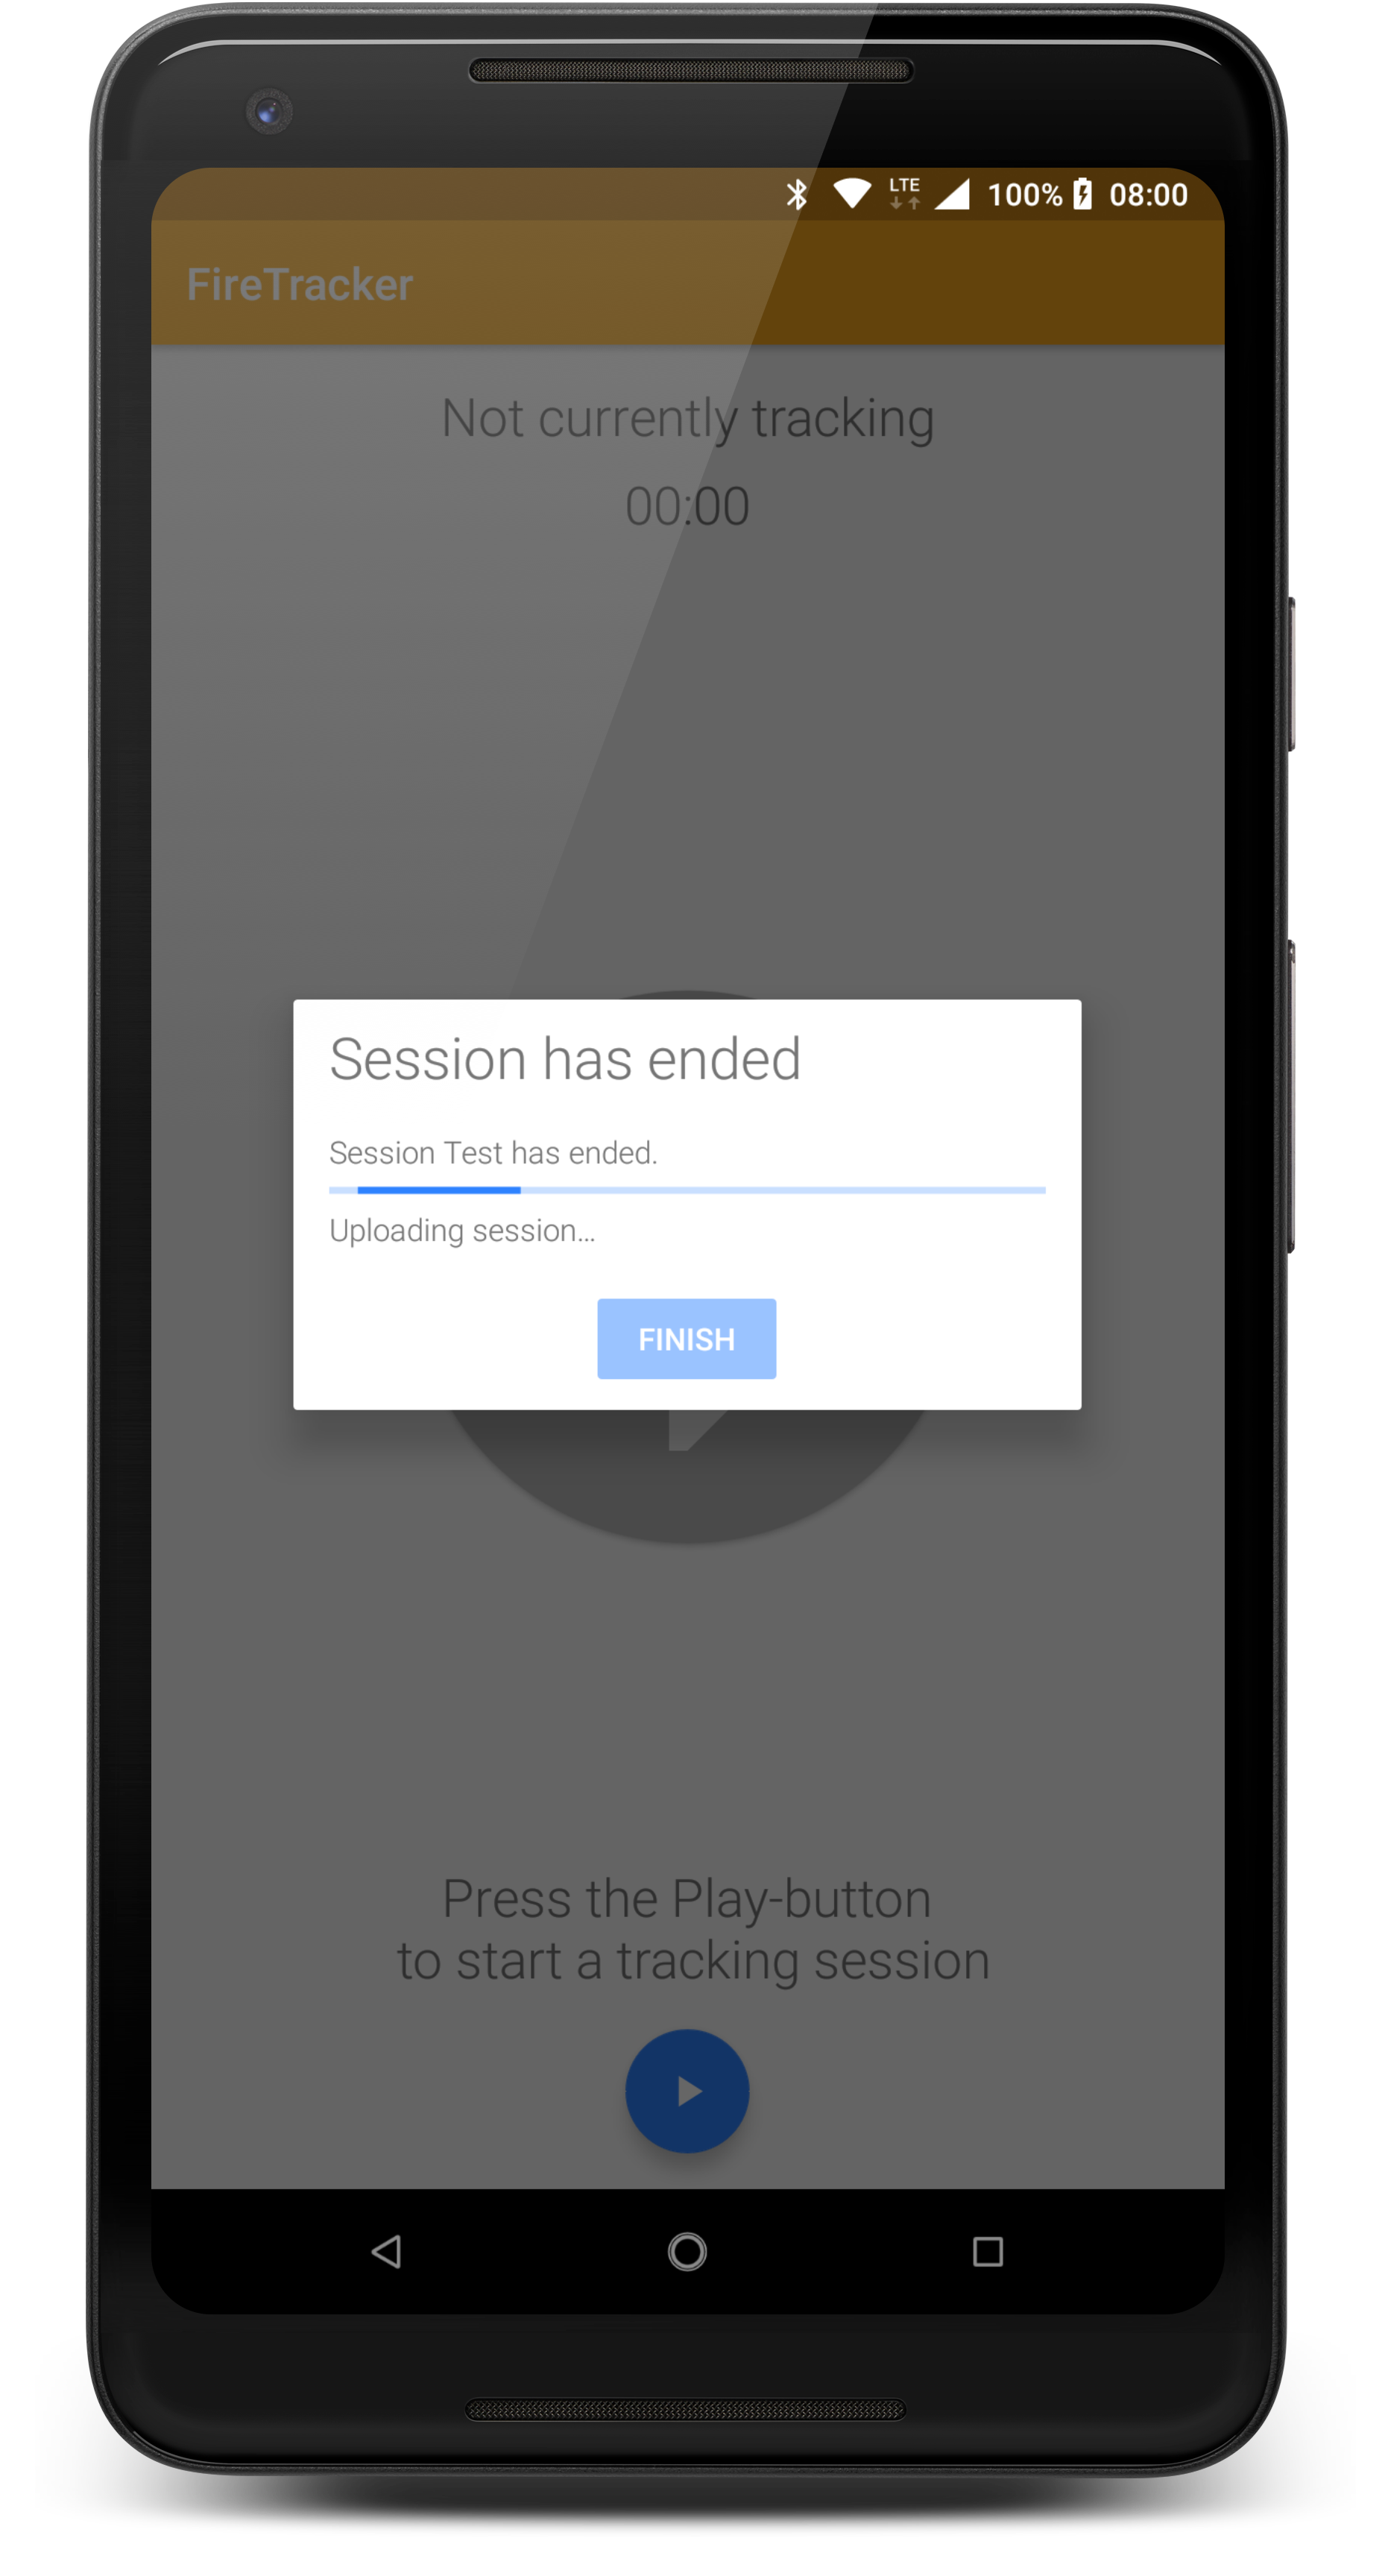
\includegraphics[width=\textwidth]{../fig/firetracker_app_old_4}
		\caption{Uploading data}
		\label{fig:app-first-prototype-upload}
	\end{subfigure}
	\caption{Screenshots of the Android application}
	\label{fig:app-first-prototype}
\end{figure}

\subsection*{Use of sensors}
In addition to tracking the Bluetooth-data the app also records data from the built-in accelerometer and gyroscope in the smartphone.
The accelerometer was used to detect movement and create an estimate of how many steps the user takes during the tracking.
This information was then used to determine if the smoke diver was walking around or standing still within a location.

The gyroscope was used to collect information about the relative orientation of the smartphone. 
The intention was to use this data to determine the orientation of the smoke diver within the building, but it turned out that different devices had different zero positioning.
Therefore, it was not possible to determine a consistent orientation across devices.
Instead the difference of orientation over a time interval was used to determine if the user rotating the device, and thereby rotating their head as the device. 

\section{Back-end}
The back-end of the FireTracker system consists of two parts.
A web-server that handles requests from the Android application and the exercise management tool, and returns data to them
An algorithm that processes the raw data from the Android app and outputs data about the locations and movements of the firefighters that can be used by the exercise management tool to create a visualization.
In this iteration the web-server functionality was implemented together with a basic processing algorithm.

\subsection{Web-server}
The web-server handles HTTP requests from the other components of the FireTracker system and stores data it receives in a database. 
It also fetches data from this database and returns it to the Android app or the exercise management tool when they ask for data.
In this iteration a variety of endpoints were implemented allowing the creation of new sessions, retrieving a list of unprocessed or processed sessions, retrieving a single unprocessed or processed session, updating an unprocessed session, adding beacons and maps, retrieving a list of beacons, and retrieving a map. 
An overview of all the endpoints is shown in Table~\ref{tab:endpoints-1}.

\begin{table}[h]
\caption{Web-server endpoints implemented in the second iteration}
\begin{tabular}{|p{0.2\linewidth}|p{0.15\linewidth}|p{0.15\linewidth}|p{0.4\linewidth}|}
\hline
\textbf{Relative path} & \textbf{Request Type} & \textbf{Parameters} & \textbf{Description}                                                    \\ \hline
/session               & OPTIONS               &                     & Create a new session                                                    \\ \hline
/raw/sessions          & GET                   &                     & Get unprocessed sessions                                                \\ \hline
/raw/session/:id       & GET                   &                     & Get a unprocessed session with the ID ``id''                            \\ \hline
/raw/sessions          & POST                  & Finished            & Get unprocessed sessions where the finished-flag is set to ``Finished'' \\ \hline
/raw/session/:id       & PUT                   &                     & Update a session with the ID ``id''                                     \\ \hline
/session/:id           & GET                   &                     & Get a processed session with the ID ``id''                              \\ \hline
/beacon                & POST                  &                     & Create a new beacon                                                     \\ \hline
/beacons               & GET                   &                     & Get a list of all beacons                                               \\ \hline
/sessionbeacon         & POST                  &                     & Create a new beacon for a specific session                              \\ \hline
/map                   & POST                  &                     & Upload a map                                                            \\ \hline
/maps/:filename        & GET                   &                     & Get the map with filename ``filename''                                  \\ \hline
\end{tabular}
\label{tab:endpoints-1}
\end{table}

\subsection{Data processing}
The data processing is executed when a session is updated with data from the tracking.
The algorithm creates a list of locations which are positions of the smoke diver at a given time.
The first location is the first data point in the list.
Then the algorithm goes through all of the remaining data points and checks if the signal is from one of the beacons used in the session. 
If the data point is from one of the associated beacons it checks if the signal is from the same beacon as the location it is currently working on.
If it is the same beacon it updates the duration of the location and checks the difference in steps and rotation values of the gyroscope to see if the walking and head movement flags should be set to true.
If it is a new beacon and it has a stronger signal strength than the last received signal from the previous beacon it creates two new locations.
The first location is an estimation of the movement of the smoke diver and is placed at the mid-point between the previous and the new beacon.
The second location is at the position of the new beacon.

\section{Data Specifications}
\label{sec:data-specifications-1}
As the three components of FireTracker need to communicate and transfer data between them, a data specification was created.
This specification was created using the JSON-standard, as the technologies used for all three components are able to create, send, receive, and use JSON-objects.

\subsection{Session}
The \textit{session-object} is an object containing all the information about a single session.\
It has an unique ID, a name, the name of the smoke diver, the start and end time of the session, a list of data points, a list of beacons used in the session, a list of generated locations, a finished-flag, and the URL to the map used for this session. 
The JSON-structure of a session, with the types of each field, is shown in Source~Code~\ref{listing:session-json-1}.

\begin{listing}[h]
	\begin{minted}
	[
	frame=lines,
	linenos
	]{json}
{
	"ID": <integer>,
	"Name": <string>,
	"User": <string>,
	"StartTime": <integer>,
	"EndTime": <integer>,
	"Datapoints": [<datapoint>],
	"Beacons": [<beacon>],
	"Locations": [<location>],
	"Finished": <boolean>,
	"Map": <string>
}
\end{minted}
\caption{Session JSON-object}
\label{listing:session-json-1}
\end{listing}

The \textit{finished-flag} is a boolean value that is set to false when the session is created, and set to true when the Android app updates it with data from the tracking.
This makes it possible to filter sessions on their finished-status so the Android app only lists sessions that have not already been used for tracking, and the exercise management tool only lists sessions that are finished and has a tracking.

\subsection{Datapoint}
A \textit{datapoint} is a registration of a single signal from a BLE beacon.
The JSON-structure of a datapoint, with the types of each field, is shown in Source~Code~\ref{listing:datapoint-json-1}.
It contains an ID, the ID of the session it is associated with, the UUID, Major and Minor of the beacon emitting the signal, a time stamp, the received signal strength index(RSSI) of the signal, the number of steps taken, and rotation-values from the gyroscope.

\begin{listing}[h]
	\begin{minted}
	[
	frame=lines,
	linenos
	]{json}
{
	"ID": <integer>,
	"SessionId": <integer>,
	"UUID": <string>,
	"Major": <string>,
	"Minor": <string>,
	"Timestamp": <integer>,
	"RSSI": <integer>,
	"Steps": <integer>,
	"RotationX": <float>,
	"RotationY": <float>,
	"RotationZ": <float>
}
\end{minted}
\caption{Datapoint JSON-object}
\label{listing:datapoint-json-1}
\end{listing}

The steps are the total number of steps the device has registered since the tracking started. 
The RotationX, RotationY and RotationZ values are the relative rotation of the device at the time of the registration of the BLE-signal.

\subsection{Beacon}
The beacon object is a representation of the BLE beacons used in the project.
It has an ID, a name, a Universally Unique Identifier (UUID), a Major value, and a Minor value.
The beacon object is used to show and select available beacons when a user creates a new session in the exercise management tool.
The JSON representation of a beacon is shown in Source~Code~\ref{listing:beacon-json-1}.

\begin{listing}[h]
	\begin{minted}
	[
	frame=lines,
	linenos
	]{json}
{
	"ID": <integer>,
	"UUID": <string>,
	"Major": <string>,
	"Minor": <string>,
	"Name": <string>
}
\end{minted}
\caption{Beacon JSON-object}
\label{listing:beacon-json-1}
\end{listing}

\subsection{SessionBeacon}
A SessionBeacon is a beacon that is used in a specific session.
It has the same fields as a beacon described in the previous section with some more information added.
The extra information is the ID of the session to which it belongs, the x-coordinate it is located at in that session, and the y-coordinate it is located at in that session.
The JSON representation of a SessionBeacon is shown in Source~Code~\ref{listing:sessionbeacon-json-1}.

\begin{listing}[h]
	\begin{minted}
	[
	frame=lines,
	linenos
	]{json}
{
	"ID": <integer>,
	"SessionId": <integer>,
	"UUID": <string>,
	"Major": <string>,
	"Minor": <string>,
	"Name": <string>,
	"XCoordinate": <float>,
	"YCoordinate": <float>
}
\end{minted}
\caption{SessionBeacon JSON-object}
\label{listing:sessionbeacon-json-1}
\end{listing}

\subsection{Location}
A \textit{location} is a position of the user at a given time during the exercise.
It is created by the data processing algorithm.
A location has an ID, the ID of the session it belongs to, an x-coordinate, an y-coordinate, a duration, a walking-flag, and a head movement-flag.
The coordinates is the coordinates of the beacon this location is associated with.
The JSON representation of a Location is shown in Source~Code~\ref{listing:location-json-1}.

\begin{listing}[h]
	\begin{minted}
	[
	frame=lines,
	linenos
	]{json}
{
	"ID": <integer>,
	"SessionId": <integer>,
	"XCoordinate": <float>,
	"YCoordinate": <float>,
	"Duration": <integer>,
	"Walking": <boolean>,
	"HeadMovement": <boolean>
}
\end{minted}
\caption{Location JSON-object}
\label{listing:location-json-1}
\end{listing}

\section{Testing}
This iteration concluded with a test of the prototype and an interview with Øygarden Fire and Rescue.

\subsection{Demonstration and testing}
The test took place at Ågotnes fire station in the office section of the building.
It started with a presentation of the prototype for the fire chief with a summary of what had been developed and how the system works.
After that the fire chief got to try out the creation of a session included placing out beacons in the building. 
A picture of him while creating the session is shown in Figure~\ref{fig:iteration2-demo}.

\begin{figure}[h]
	\centering
	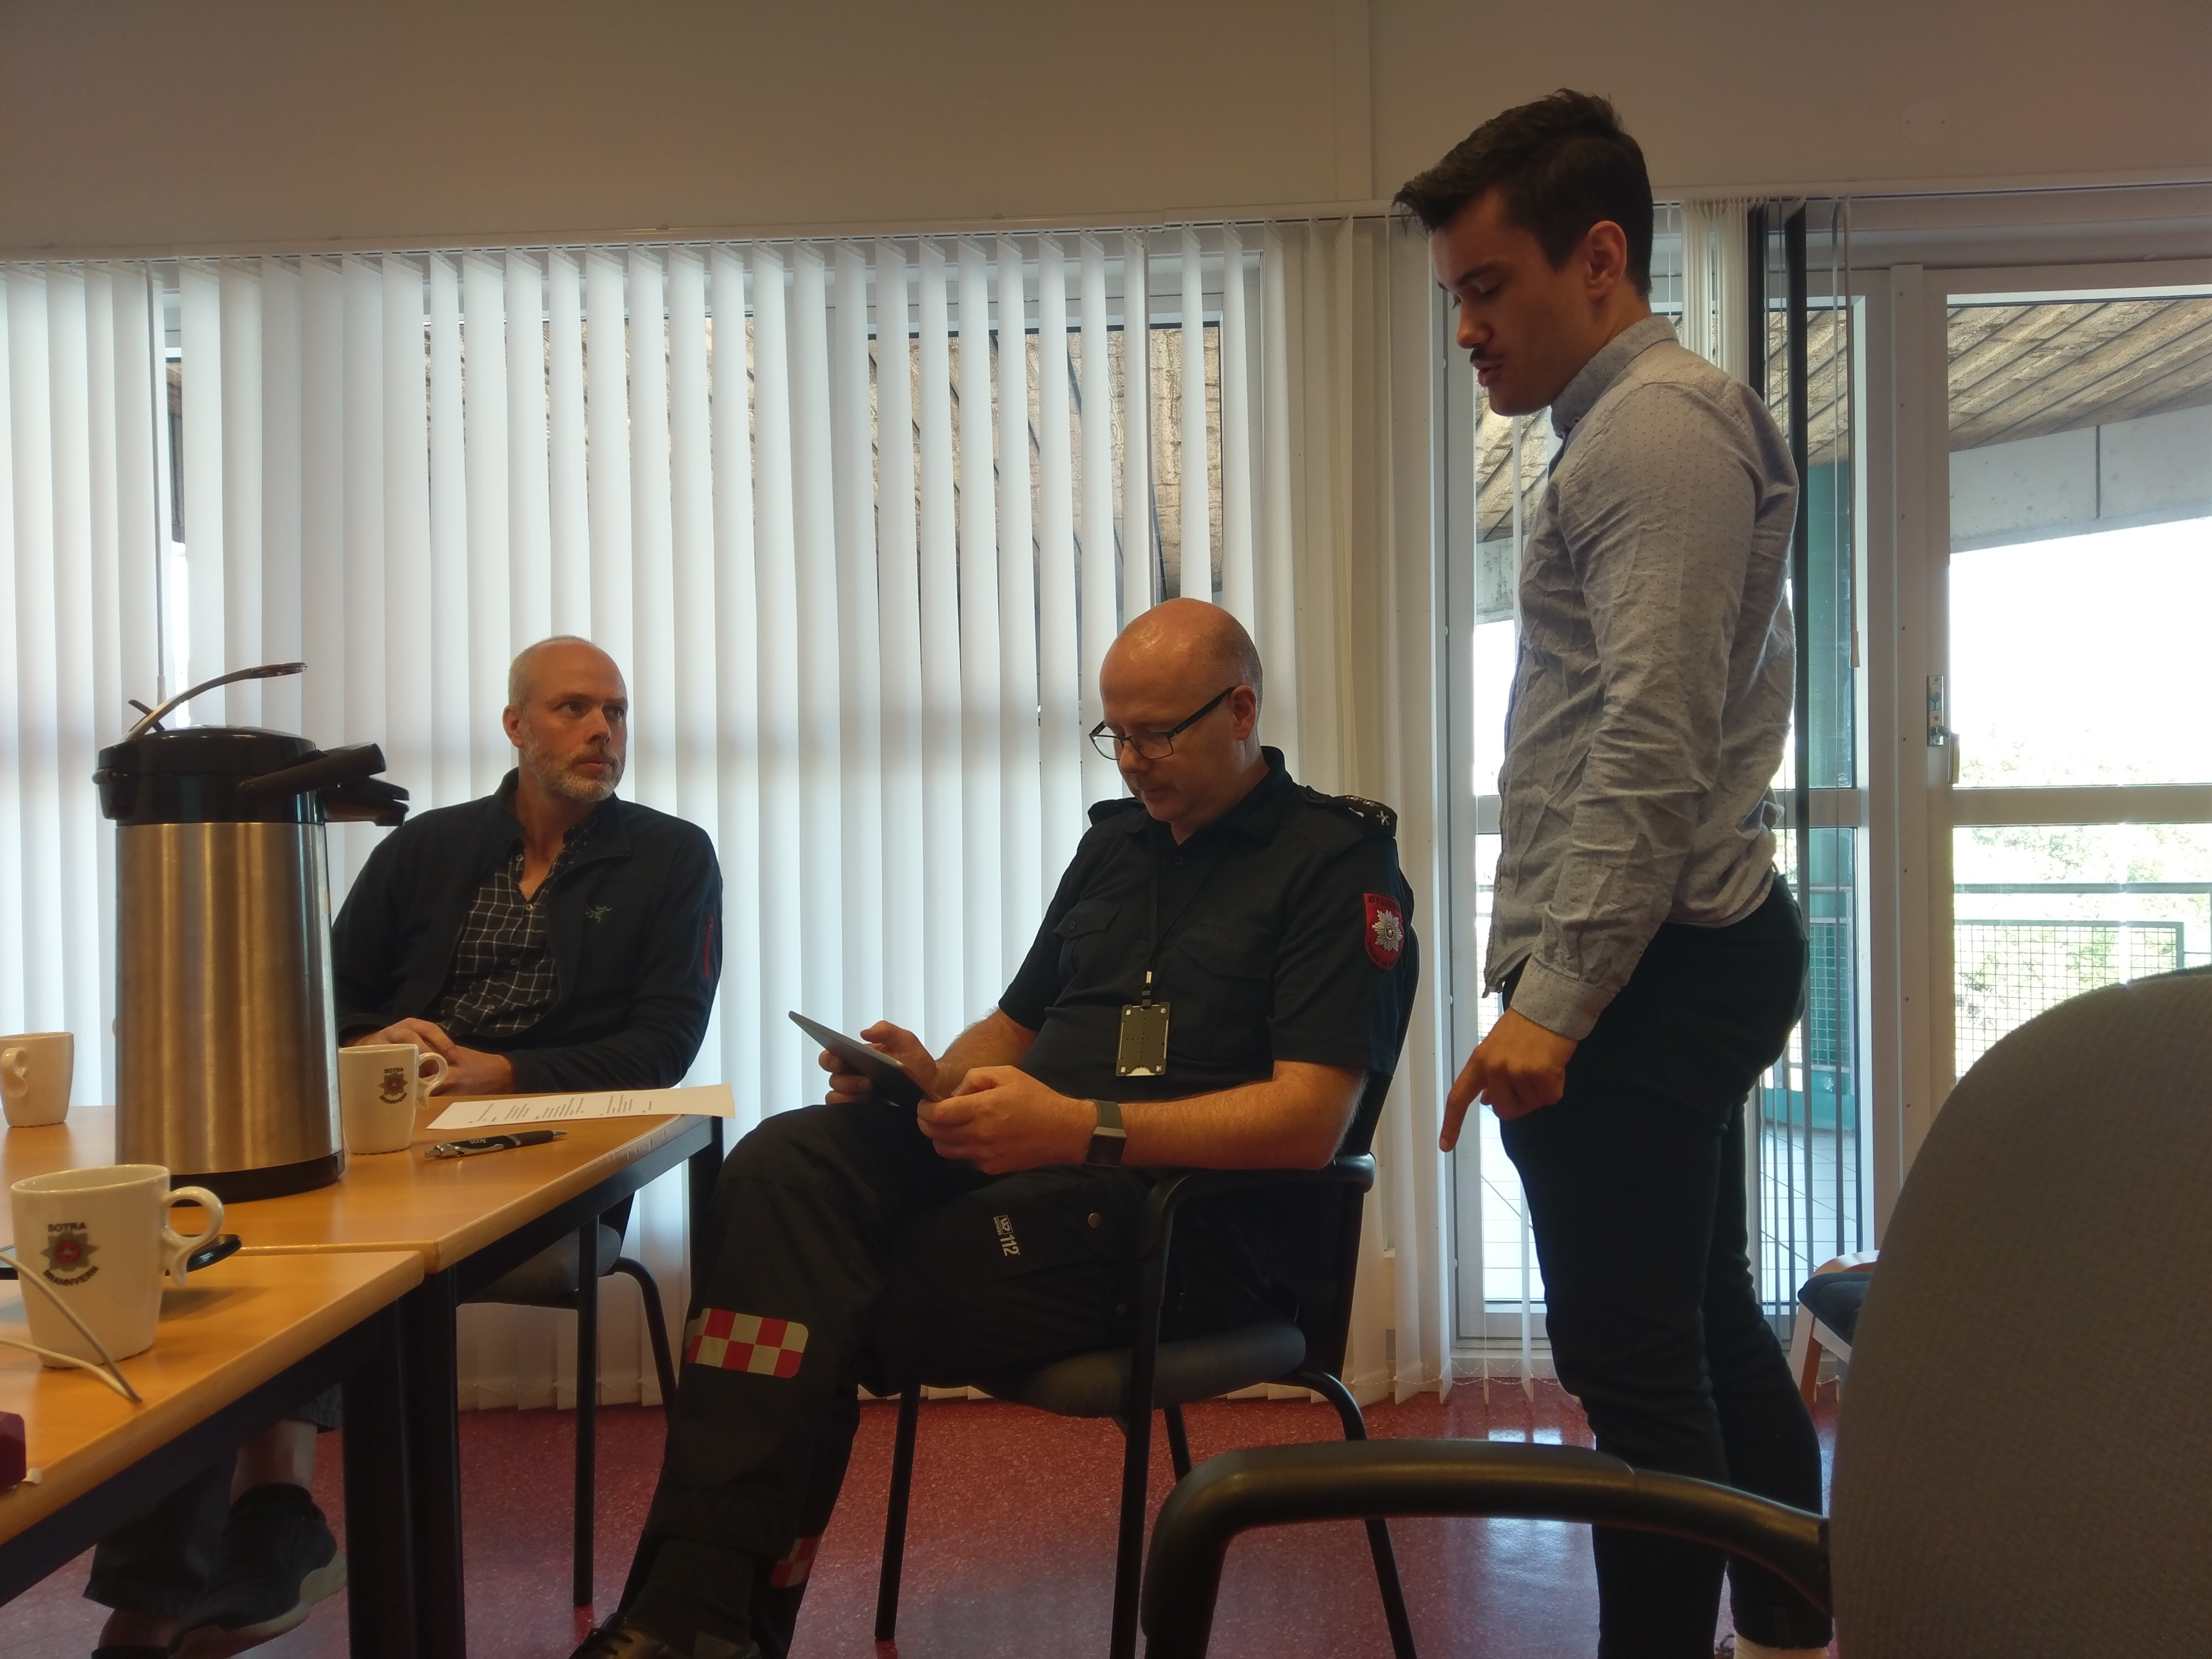
\includegraphics[width=\textwidth]{../fig/iteration2-demo}
	\caption[Fire chief testing the FireTracker system]{Fire chief (sitting in the middle) testing the FireTracker system}
	\label{fig:iteration2-demo}
\end{figure}

When the session was created and all the beacons were placed the fire chief started up the Android app and selected the session he created and started tracking.
With the tracker active he walked slowly through the upper floor where all the beacons was placed.
After he had finished walking through the building he ended the session and uploaded the data.
The generated visualization was then showed to him.
This visualization is shown in Figure~\ref{fig:iteration2-map}.

\begin{figure}[h]
	\centering
	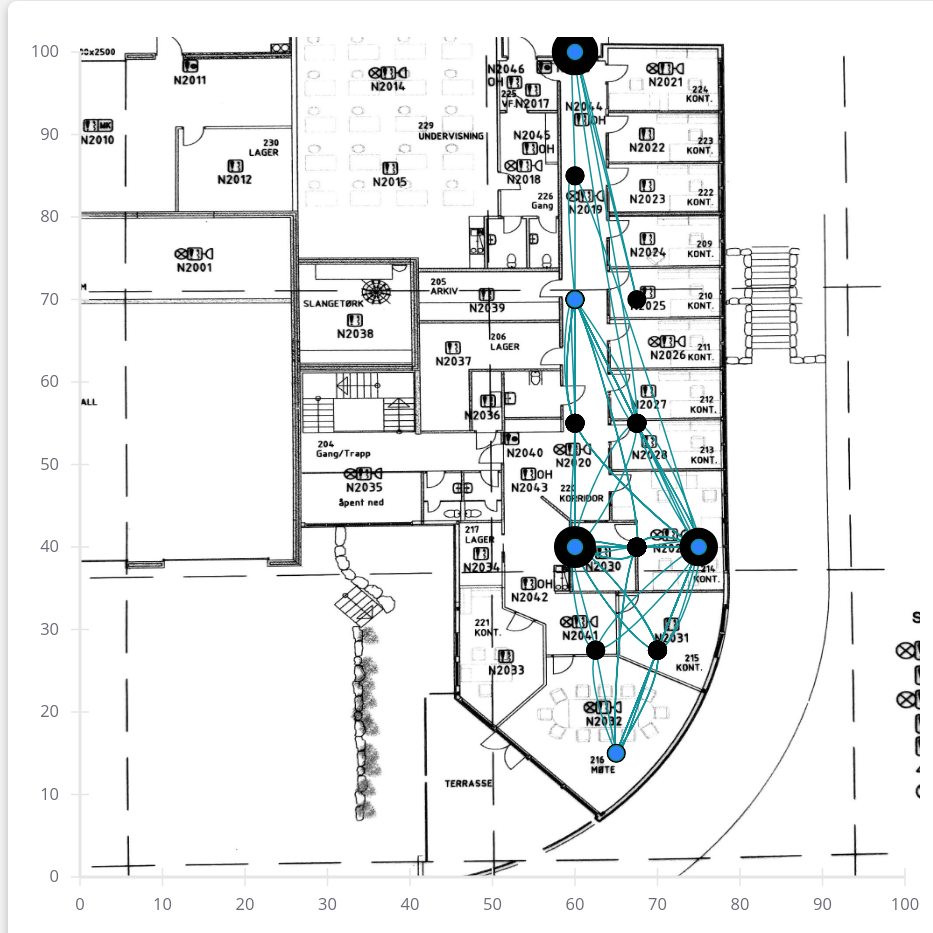
\includegraphics[width=\textwidth]{../fig/iteration2-map}
	\caption{Map with tracking from test in iteration 2}
	\label{fig:iteration2-map}
\end{figure}

In the visualization the blue dots are the position of the beacons.
The black dots are the visited locations, including the estimated midway points.
The blue lines are the movements between locations.

In this test five beacons were used. 
The beacons were borrowed from another project, as the beacons intended for this project were not yet available.
The borrowed beacons where two different models from Estimote.
Three of them were placed in a straight hallway, one was placed in an office in the bottom right (on the figure) end of the hallway, and one was placed in a meeting room next to the end of the hallway.
The tracking began in the upper end of the hallway, and he walked through the hallway, into the office, back to the hallway, and into the meeting room where the tracking ended.

When he was testing the visualization in the exercise management tool the fire chief said that it felt very cluttered because of all the points and lines.
He would have preferred to not have the estimated mid-points between two locations, and rather used more beacons with a shorter range.
The reason for all the lines in the graph is probably both because the beacons used for this test were transmitting using different, and too strong, signal strength, and because many of them were placed in the same room.
Using beacons transmitting with a lower signal-strength, and therefore having a shorter range, would probably solve aspects of this problem as well.

\subsection{Interview}
After the test the fire chief was interviewed using a semi-structured interview.
The interview lasted for 30 minutes and was transcribed afterwards.
The interview guide is included in Appendix~\ref{app:interview-guide-second}.

The questions for the interview was divided into four categories: practical, user interface, visualization, and data.

\subsubsection*{Practical}
\begin{itemize}
	\item How was it to set up a session?
\end{itemize}

\textbf{Summary of answer:}\\
\textit{Setup:}
It was easy both to understand and create a session. 
It was really easy to take a picture of the map, upload it and place the beacons on the map.

\subsubsection*{User Interface}
\begin{itemize}
	\item Were there parts of the system that was difficult to understand or use?
	\item Does the system (app+exercise management tool) give enough information on how to use it?
\end{itemize}

\textbf{Summary of answers:}\\
\textit{Difficulty:}
It was easy to use. 
The fire chief got the first presentation of the system less than an hour before the setup and has already created and used a session without problems.

\textit{Use Information:}
The fire chief meant that there should be a user manual for the system that can be read before using the system. 
If that user manual explains the process simply and with pictures it should be no problem to use the system.
They would also prefer to have the system entirely in Norwegian. 

\subsubsection*{Visualization}
\begin{itemize}
	\item How was the navigation of the visualization?
	\item Did you get enough information about the session?
	\item Was there anything in the graph or map that was unclear?
	\item What could the visualization in its current condition be used for?
\end{itemize}

\textbf{Summary of answers:}\\
\textit{Navigation:}
Navigation was a bit challenging to begin with.
It would have been easier if everything was onscreen at the same time to avoid having to scroll up and down.
It looked okay on the PC, but on the iPad, which is what they are going to use, it was some scrolling.

\textit{Enough Information:}
The duration of each location, together with their placement on the map, can be used to discuss why the smoke divers spent much or little time in different parts of the building.

\textit{Unclear:}
The fire chief thought the map was very clear, except for the number of dots and lines in the graph.
As he set up the session one could wonder if it might be a bit harder for someone else to understand, because of all the dots and lines.

\textit{Visualization:}
In the current state it would be hard to interpret and use the visualization because of the large number of points in the graph.


\subsubsection*{Data}
\begin{itemize}
	\item What do you think about using information on head movement to say something about how active a firefighter is?
	\item We use step counter to see if a smoke diver moves inside the area of a beacon. Is this information interesting?
	\begin{itemize}
		\item Would it be interesting to show the number of steps or the distance?
	\end{itemize}
\end{itemize}

\textbf{Summary of answers:}\\
\textit{Head Movement:}
Using head movement to indicate activity could end up being too much data as the smoke divers use their bodies actively and are in constant movement.
The fire chief meant that the most important and interesting information is the tracing of their location.

\textit{Step Counter:}
The fire chief thought that it could be interesting to show the number of steps walked as the smoke divers are supposed to use their feet actively in the search, and this could be an indicator on how much they used their feet.

\subsection{Analysis of interview}
It is clear that the fire department is interested in using a system such as FireTracker, and they think it could be a valuable form of feedback when evaluating smoke diving exercises.
The system is easy to understand and use, and with the addition of in-system instructions, it would be even better.
At the moment the problem with the system is the large amount of points in the visualization, which are caused by the estimated mid-points between two locations.
Those should be removed to reduce the clutter.

\section{Summary}
This chapter has described the second iteration of the development process.
In this iteration a working prototype of the system was developed, and tested together with Øygarden Fire and Rescue.
The new requirements for the next iteration are:
\begin{itemize}
	\item Reduce information in the visualization
	\item Use Norwegian everywhere in the system
	\item Add safety features to prevent data loss
\end{itemize}

\end{document}
